\section{Introduction}

%% Background
Wide-area streaming analytics are becoming pervasive, especially with emerging
Internet of Things (IoT) applications. Large cities such as London and Beijing
have deployed millions of cameras for surveillance and traffic
control~\cite{skynet, london.surveillance}. Buildings are increasingly equipped
with a wide variety of sensors to improve energy efficiency and occupant
comfort~\cite{krioukov2012building}. Geo-distributed infrastructure, such as
content delivery networks (CDNs), analyze requests from machine logs across the
globe~\cite{mukerjee2015practical}. These applications all transport, distill,
and process streams of data across the wide area, in real time.

A key challenge that the above applications face is dealing with the scarce and
variable bandwidth in the wide area~\cite{hsieh17gaia, vulimiri2015global}.  As
many have observed, WAN bandwidth growth has been decelerating for many years
while traffic demands are growing at a staggering
rate~\cite{global2016telegeography, cisco2013zettabyte, cisco2016global}.  In
addition, scarcity in last-mile bandwidth remains a problem across
wireless~\cite{biswas2015large}, cellular~\cite{nikravesh2014mobile}, and even
broadband~\cite{grover2013peeking, sundaresan2014bismark} networks.  Finally, as
we elaborate on in \autoref{sec:motivation}, not only is WAN bandwidth scarce,
it is also relatively expensive, and highly variable.

For all of the above reasons, it is important that streaming applications be
\emph{adaptive}, incorporating the ability to optimally trade-off accuracy for
bandwidth consumption and hence a key system challenge is to design the
\emph{programming abstractions and tools} that simplify the development of such
adaptive applications.

In recent years, systems such as Storm~\cite{toshniwal2014storm}, Spark
Streaming~\cite{zaharia2013discretized}, and VideoStorm~\cite{zhang2017live},
have emerged in support of stream processing.  These systems enable efficient
processing of large streams of data, but are designed to work within a single
datacenter cluster (where network bandwidth is typically not the bottleneck) and
hence they do not focus on support for adapting to the vagaries of WAN
bandwidth.

Recent research on WAN-aware systems promote pushing computation to the network
edge~\cite{rabkin2014aggregation, satyanarayanan2009case}.  However, even with
edge computing, the need for adaptation remains because end-devices such as
cameras and mobile phones still suffer from limited bandwidth in the last-hop
infrastructure~\cite{abari2017enabling, zhang2015design}.  In addition, edge
computing is not a panacea as wide-area communication is often not entirely
avoidable: e.g., some analytical jobs require joining or aggregating data from
multiple geo-distributed sites~\cite{pu2015low, viswanathan2016clarinet}, while
in some cases processing benefits substantially from specialized computing
resources such as GPUs and TPUs~\cite{abadi2016tensorflow} in the cloud.

The core difficulty with adaptive streaming analytics is that, when bandwidth is
scarce, developers are faced with the decision of how to reconcile data fidelity
(i.e., not losing any data) with data freshness (i.e., sending data as quickly
as possible). A deterioration in either fidelity or freshness can impact
application accuracy but the exact impact varies depending on the
application.\footnote{E.g., an application tracking the current value of a
  variable might prioritize freshness while one that is computing an average
  might prioritize fidelity.} \autoref{fig:intro} illustrates this trade-off
with a few sample points in the design space.

\begin{figure}
  \centering
  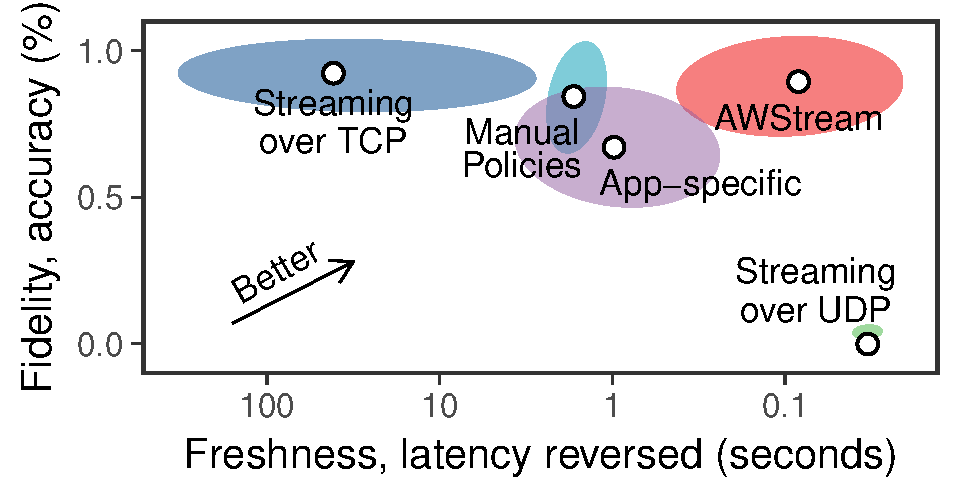
\includegraphics[width=0.8\columnwidth]{figures/figure1.pdf}
  \caption{The trade-off space between data freshness and fidelity when facing
    insufficient bandwidth (details in \autoref{sec:runtime-adaptation}).}
  \label{fig:intro}
  \vspace{-1em}
\end{figure}

Applications that simply use existing protocols without any attempt at
adaptation can result in extreme design points. E.g., streaming over TCP ensures
reliable delivery (hence high fidelity) but backlogged data delays the delivery
of data (hence freshness suffers).  On the other hand, streaming over UDP
minimizes latency by sending packets as fast as possible, but uncontrolled
packet loss can devastate data fidelity.

Manual policies, such as sampling, allow developers to trade data fidelity for
freshness~\cite{rabkin2014aggregation}. However, it's difficult to write
accurate policies without extensive domain expertise or considerable effort. In
practice, developers write manual policies based on heuristics rather than
quantitative measurements and, as we show in \autoref{sec:evaluation}, such
policies can lead to sub-optimal performance in terms of both freshness and
fidelity.

Furthermore, application-specific optimizations often do not generalize. A
fine-tuned adaptation algorithm for one application works poorly for a different
application, if performance metrics or data distributions change.  For example,
video streaming focuses on quality of experience
(QoE)~\cite{michalos2012dynamic, pantos2016http, yin2015control}. Because humans
favor smoothness over image quality, these systems maintain a high frame rate,
e.g.\,\(25~\text{FPS}\), and reduce the resolution under bandwidth limitation.
However, low resolution images can lead to poor accuracy for video analytics
that rely on the image details, e.g.\,face detection~\cite{viola2001rapid}.

In this paper, we present \sysname{}, a framework for building adaptive stream
processing applications that simultaneously simplifies development \emph{and}
improves application accuracy in the face of limited or varying wide-area
bandwidth.
% for the wide area that achieves low latency and high accuracy simultaneously
% with minimal developer effort.
\sysname{} achieves this through the combination of three novel contributions:

\begin{enumerate}[leftmargin=*]
\item \sysname{} introduces new programming abstractions by which a developer
  expresses \emph{what} degradation functions can be used by the framework.
  % {\bf Sylvia: Cut remainder of para? Too much detail for intro?}  More
  % specifically, \sysname{} augments existing stream processing operators with
  % a new \maybe{} operator. Its basic form takes a function that degrades the
  % input stream, and a list of values that serve as a knob to control the level
  % of degradation.  and . The knob specifies the degradation level that affects
  % data size and data fidelity.  We extend the basic form with a library of
  % specialized operators for common data types, such as
  % \texttt{maybe\_downsample} for images.  Our API is \textit{composable}
  % (multiple operators form a configuration that affects the adaptation
  % jointly), and \textit{extensible} (arbitrary functions and external
  % libraries can be embedded with our operators).
  Importantly, developers do not have to specify exactly when and how different
  degradation functions are to be used which is instead left to the \sysname{}
  framework.

\item Rather than rely on manual policies, \sysname{} automatically
  \emph{learns} a Pareto-optimal policy or strategy for when and how to invoke
  different degradation functions.  For this, we design a methodology that uses
  a combination of offline and online training to build an accurate model of the
  relationship between an application's accuracy and its bandwidth consumption
  under different combinations of degradation functions. Our solution exploits
  parallelism and sampling to efficiently explore the configuration space and
  learn an optimal strategy.

  % The key idea is to \textit{automatically} build an accurate and precise
  % \textit{performance model} instead of relying on manual policies or
  % application-specific optimizations.
  % We use an \textit{offline} process to bootstrap our system with
  % developer-supplied training data, and continuously refine the profile
  % \textit{online} to handle \textit{model drift}.  We exploit parallelism and
  % sampling-based techniques to efficiently explore the configuration space and
  % learn a adaptation strategy.

\item \sysname{}'s final contribution is the design and implementation of a
  runtime system that continually measures and adapts to network conditions.
  \sysname{} matches the streaming data rate to the measured available
  bandwidth, and achieves high accuracy by using the learned Pareto-optimal
  configurations.  Upon encountering network congestion, our adaptation
  algorithm increases the degradation level to reduce the data rate, such that
  no persistent queue builds up. To recover, it progressively decreases the
  degradation level after probing for more available bandwidth.

  % The runtime also provides additional options to control application
  % behaviors, such as limiting the maximum
  % allowed WAN bandwidth. For multiple applications, the profiles can be used
  % to allocate bandwidth among competing tasks for \textit{utility fairness}.
\end{enumerate}

We implement \sysname{} and use it to prototype three streaming applications:
augmented reality (AR), pedestrian detection (PD), and distributed Top-K
(TK). We use real-world data to profile these applications and evaluate their
runtime performance on a geo-distributed public cloud.  We show that
\sysname{}'s data-driven approach generates accurate profiles and that our
parallelism and sampling techniques can speed up profiling by up to 29$\times$
and 8.7$\times$\@ respectively.

We show that \sysname{} significantly outperforms non-adaptive applications:
e.g., achieving a 40--100$\times$ reduction in packet delivery times relative to
applications built over TCP, or an over 45--88\% improvement in data fidelity
(application accuracy) relative to applications built over UDP.  We also compare
\sysname{} to JetStream~\cite{rabkin2014aggregation}, a state-of-the-art system
for building adaptive streaming analytics that is based on manual policies: our
results show that besides the benefit of generating optimal policies
\textit{automatically}, \sysname{} achieves a 15-20$\times$ reduction in latency
and 1-5\% improvement in accuracy relative to JetStream. We show that these
gains come from the combination of \sysname{}'s ability to learn better policies
\emph{and} its well-designed runtime.  Hence, the ease of development that
\sysname{} provides comes with significantly \emph{improved} application
performance compared to typical manually crafted policies.

%%% Local Variables:
%%% mode: latex
%%% TeX-master: "../awstream"
%%% End:

%% LocalWords: VideoStorm analytics CDN CDNs geo IoT TCP UDP QoE runtime
%% LocalWords: GPUs TPUs downsample composable TK JetStream datacenter